\documentclass{beamer}
\usepackage{hyperref}
\hypersetup{
	colorlinks,
	citecolor=white,
	filecolor=white,
	linkcolor=white,
	urlcolor= cyan
}

\usetheme[progressbar=foot, background=dark]{metropolis}  
\setbeamertemplate{frame footer}{Ankit Pant, Harshita Agrawal, Ravi Jakhania}

\title{\centering Distributed Systems Project\\ \vspace{2mm} \normalsize{Simulate message delivery guarantees such as FIFO and Arbitrary, and their impact on some Mutual Exclusion Distributed Algorithm  } \\ \vspace{-5mm}}
\author{Ankit Pant  2018201035 \\ 
		Harshita Agrawal 2018201014 \\
		Ravi Jakhania 2018201018 }
\date{}
\begin{document}
\begin{frame}[plain]
    \maketitle
\end{frame}
\begin{frame}{Outline}
	\setbeamertemplate{section in toc}[sections numbered]
	\tableofcontents
\end{frame}

\section{Introduction}
	\begin{frame}{Introduction}
		\begin{itemize}
			\item Distributed systems are quite ubiquitous these days
			\item Communication between nodes should be robust
			\item  Need a layer of dependable software systems for reliable communication
			\item This project aims to explore and simulate two modes or channels of communication
			\begin{itemize}
				\item First In First Out or \emph{FIFO} message ordering channels
				\item \emph{Arbitrary} message ordering channels
			\end{itemize}
			\item We simulate Lamport's Mutual Exclusion Algorithm and measure impact on both message ordering channels
		\end{itemize}
	\end{frame}

\section{Literature Review}
	\begin{frame}{Message Ordering and Group Communication}
		\begin{itemize}
			\item Group communication is vital in Distributed Systems
			\item Order in which the messages are delivered is also important
			\begin{itemize}
				\item It determines the order of execution of commands and also helps with consistency
			\end{itemize}
			\item Arbitrary Order
			\begin{itemize}
				\item No ordering between messages sent by one node to the other
				\item Also called \textit{non-FIFO}
				\item \textbf{Example:} If a process `P1' sends two messages (m1 and m2) to `P2' and the timestamp of message \textit{m1} is \textit{t1} and for message \textit{m2} is \textit{t2} where $t1<t2$ the process `P2' may either receive message \textit{m1} before message \textit{m2} or it may receive message \textit{m2} before message \textit{m1}
			\end{itemize}
		\end{itemize}
		
	\end{frame}

	\begin{frame}{Message Ordering and Group Communication}
		\begin{itemize}
			\item FIFO Order
			\begin{itemize}
				\item Messages sent by a process to another is received in the same order that they were sent
				\item \textbf{Example:} If a process `P1' sends two messages (m1 and m2) to `P2' and the timestamp of message \textit{m1} is \textit{t1} and for message \textit{m2} is \textit{t2} where $t1<t2$ the process `P2' must necessarily receive message \textit{m1} before message \textit{m2}
				\item Relative ordering between multicast messages from different senders is not important
			\end{itemize}
		\end{itemize}
		
	\end{frame}

		%\begin{frame}{Message Ordering and Group Communication}
		%\begin{itemize}
		%	\item Causal Order
		%	\begin{itemize}
		%		\item If two send (or more) events happen then their corresponding receive events happen in the same order as well throughout the distributed system
		%		\item Stricter version of \textit{FIFO} ordering
		%		\item Relative ordering between multicast messages from different senders is also taken into account
		%		\item \textbf{Example:} If there are two messages \textit{m1} and \textit{m2} then if send timestamp of \textit{m1} $<$ send timestamp of \textit{m2}, then for each destination of those messages, receive timestamp of \textit{m1} $<$ receive timestamp of \textit{m2}
		%	\end{itemize}
	%	\end{itemize}
		
	%\end{frame}
	
	
		\begin{frame}{Distributed Mutual Exclusion Algorithm}
		\begin{itemize}
			\item Mutual exclusion -- one of the core problems 
			\item More than two nodes should not be executing critical section at the same time
			\item No shared memory $\implies$ semaphores, etc. not possible
			\item Distributed mutual exclusion algorithms implemented as
			\begin{itemize}
				\item Token based algorithms
				\item Non-token based approach
				\item Quorum based approach
			\end{itemize}
		\end{itemize}
		
	\end{frame}

	\begin{frame}{Lamport's algorithm}
		\begin{itemize}
			\item Token based Distributed Mutual Exclusion Algorithm
			\item Executes the critical section requests from various processes in the increasing order of timestamps
			\item Every node keeps a queue called the \textit{request queue}
			%\item Requires FIFO ordered channel to execute correctly
			\item Phases of Lamport's algorithm:
			\begin{itemize}
				\item Requesting the critical section
				\item Executing the critical section
				\item Releasing the critical section
			\end{itemize}
		\end{itemize}
		
	\end{frame}
	
	\begin{frame}{Lamport's algorithm (Pseudocode)}
		\begin{figure}[H]
			\label{Lamportalgo}
			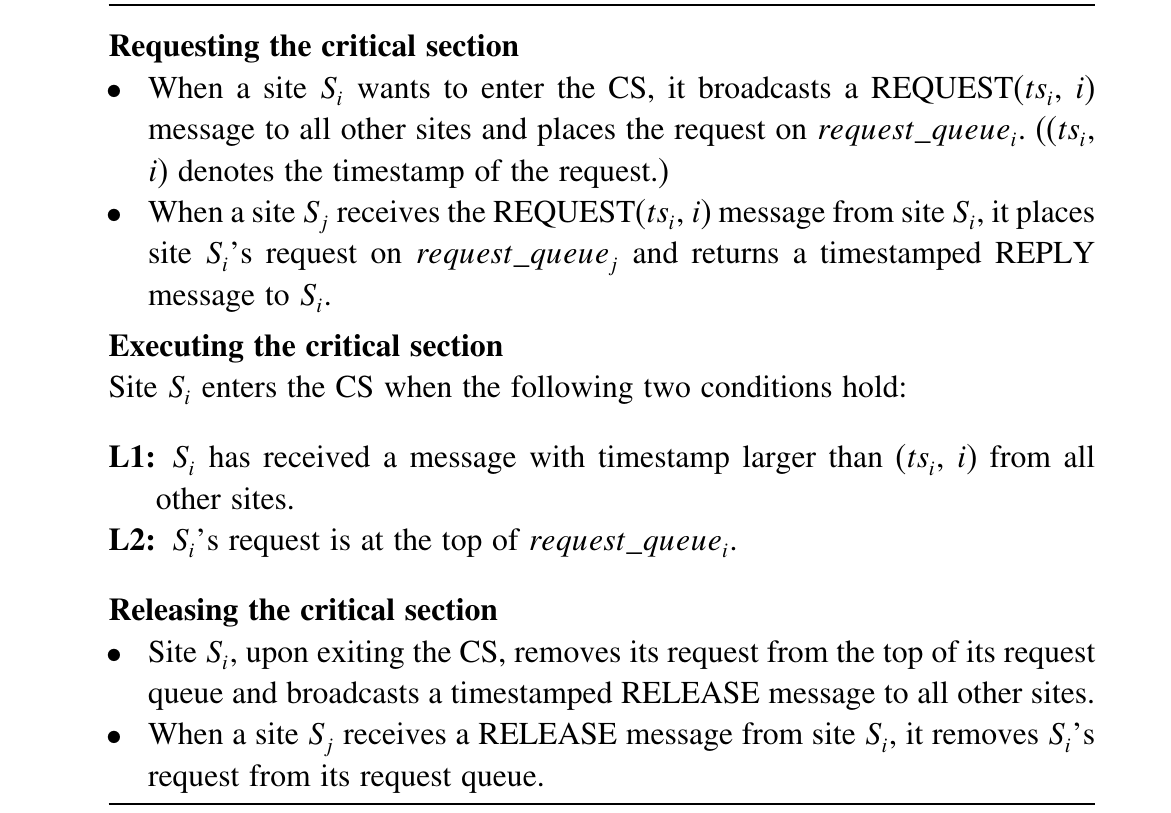
\includegraphics[width=90mm]{lamport_algo.png}
			\caption{Pseudocode for Lamport's Algorithm \cite{4}}
		\end{figure}
		
	\end{frame}
	
	



\section{Methodology}
	\begin{frame}{System Model}
		\begin{itemize}
			\item Simulated Distributed System with 6 nodes
%			\item Nodes and channel assumed to be reliable (since it is precondition to run Lamport's algorithm)
			\item All nodes are non-Byzantine
			\item Message delivery guaranteed by using TCP as underlying protocol
			\item Each node in the system can (pre-requisites of Lamport's algorithm)
			\begin{itemize}
				\item Send and receive messages
				\item Request to execute its critical section
				\item Communicate with every other node
			\end{itemize}
			\item Nodes (channels) may arbitrary fail and come back online (handled using timeouts)
		\end{itemize}
	\end{frame}


\section{Code Walkthrough}
	\begin{frame}{Source Code}
		\Large{Please refer to the source code and accompanying video for details on the source code}
	\end{frame}	



\section{Experimentation and Results}
	\begin{frame}{Results}
		\begin{itemize}
			\item \textit{FIFO} message ordering was successfully implemented
			\item \textit{Arbitrary} message was successfully implemented
			\item Lamport's algorithm was run on both the ordered channels
			\item Lamport's algorithm runs correctly on \textit{FIFO} ordered channel
			\item Lamport's algorithm fails on \textit{Arbitrary} ordered channel
			\item In both message ordering channels the number of messages exchanged is same [$3*(N-1)$]
			\item Runtime not measured due to random delays in network (can cause inaccurate assessment)
		\end{itemize}
	\end{frame}
	

\section{Conclusion}
	\begin{frame}{Conclusion}
		\begin{itemize}
			\item Message ordering is crucial for correct working of distributed algorithms
			\item Maintaining Mutual exclusion is also vital in a distributed system
			\item Lamport's algorithm may fail in an \textit{Arbitrary} ordered channel
		\end{itemize}
	\end{frame}


\section{Future Scope}
	\begin{frame}{Future Scope}
		\begin{itemize}
			\item Lamport's algorithm can be modified to run on \textit{Arbitrary} channels
			\item Resolution may be done by
			\begin{itemize}
				\item Adding buffer at receivers
				\item Buffer orders messages correctly by timestamp
				\item After all messages are received and correctly ordered, forward them to the mutual exclusion algorithm
			\end{itemize}
		\end{itemize}
	\end{frame}
	

\section{References}
	\begin{frame}[allowframebreaks]{References}
		
		\begin{thebibliography}{4}
		\bibitem{1} \textit{FIFO executions}, Ajay D. Kshemkalyani \& Mukesh Singhal, Page 191, Distributed Computing Principles, Algorithms, and Systems.
		\bibitem{2} \textit{Causally ordered (CO) executions}, Ajay D. Kshemkalyani \& Mukesh Singhal, Page 191, Distributed Computing Principles, Algorithms, and Systems.
		\bibitem{3}\textit{Distributed mutual exclusion algorithms}, Ajay D. Kshemkalyani \& Mukesh Singhal, Page 305, Distributed Computing Principles, Algorithms, and Systems.
		\bibitem{4}\textit{Lamport's Algorithm}, Ajay D. Kshemkalyani \& Mukesh Singhal, Page 309, Distributed Computing Principles, Algorithms, and Systems.
		
		\end{thebibliography}
	
	\end{frame}

\end{document}
